\def \currentAuthor {} %so kann jederzeit der Autor geändert werden -> wird in der Fusszeile angezeigt.

\chapter*{Einleitende Bemerkungen}

\chapter*{Notationen}
Beschreibung wie Code, Hinweise, Zitate etc. formatiert werden  

\chapter{Einleitung}

\chapter{Projektmanagement}

\section{Metainformationen}
\subsection{Team}
\subsection{Betreuer}
\subsection{Partner}
\subsection{Ansprechpartner}
\section{Vorerhebungen}
\subsection{Projektzieleplan}
Projektziele-Hierarchie - SMART
\subsection{Projektumfeld}
\begin{itemize}
	\item Identifikation der Stakeholder
	\item Charakterisierung der Stakeholder
	\item Maßnahmen
	\item Grafische Darstellung des Umfeldes
\end{itemize}
\subsection{Risikoanalyse}
\begin{itemize}
	\item Risikomatrix
\end{itemize}
\section{Pflichtenheft}
\subsection{Zielbestimmung}
\begin{itemize}
	\item Projektbeschreibung
	\item IST-Zustand
	\item SOLL-Zustand
	\item NICHT-Ziele (Abgrenzungskriterien)
\end{itemize}
\subsection{Produkteinsatz und Umgebung}
\begin{itemize}
	\item Anwendungsgebiet
	\item Zielgruppen
	\item Betriebsbedingungen
	\item Hard-/Softwareumgebung
\end{itemize}
\subsection{Funktionalitäten}
\begin{itemize}
	\item MUSS-Anforderungen
	\begin{itemize}
		\item Funktional
		\item Nicht-funktional
	\end{itemize}
	\item KANN-Anforderungen
	\begin{itemize}
		\item Funktional
		\item Nicht-funktional
	\end{itemize}
\end{itemize}
\subsection{Testszenarien und Testfälle}
\begin{itemize}
	\item Beschreibung der Testmethodik
	\item Testfall 1
	\item Testfall 2
	\item \ldots
\end{itemize}
\subsection{Liefervereinbarung}
\begin{itemize}
	\item Lieferumfang
	\item Modus
	\item Verteilung(Deployment)
\end{itemize}
\section{Planung}
\subsection{Projektstrukturplan}
\def \currentAuthor{Florian Tipotsch}
\newpage
\begin{table}[H]
	\centering
	\caption{Projektstrukturplan}
	\label{projektstrukturplan}
	\begin{tabular}{lll}
		P 1   & Projektstart                     &                                \\
		1     & Planung                          & Alle                           \\
		1.1   & Besprechungstermine setzen       & Alle                           \\
		1.1.1 & Vertrag erstellen                & Alle                           \\
		1.2   & Verantwortungsmatrix             & Alle                           \\
		1.3   & Budgetplan erstellen             & Alle                           \\
		2     & Programmierung (Kevin + Flo)     & Kevin Glatz, Florian Tiptsch   \\
		2.1   & Programmiersprache               & Kevin Glatz                    \\
		2.1.1 & Sprache Wählen Š                 & Kevin Glatz                    \\
		2.1.2 & Informationsammlung für Features & Kevin Glatz                    \\
		2.1.3 & Vertraut machen                  & Kevin Glatz                    \\
		2.2   & Arduino UNO kaufen (Flo)         & Florian Tipotsch               \\
		2.2.1 & Vertraut machen                  & Kevin Glatz                    \\
		2.2.2 & Test Programme                   & Kevin Glatz                    \\
		2.3   & Programmierung des Brutkasten    & Kevin Glatz                    \\
		3     & Brutkasten (Leo)                 & Leonid Hammer                  \\
		3.1   & Equipment Liste erstellen        & Leonid Hammer                  \\
		3.1.1 & Equipment überprüfen             & Leonid Hammer                  \\
		3.1.2 & Equipment Kaufen                 & Alle                           \\
		3.2   & Konzeptzeichnung                 & Leonid Hammer                  \\
		3.2.1 & Zeichnen                         & Leonid Hammer                  \\
		3.2.2 & Bauen                            & Leonid Hammer                  \\
		
		4     & Datenbank                        & Kevin Glatz                    \\
		4.1   & ER-Diagramm                      & Florian Tipotsch + Kevin Glatz \\
		4.2   & Sprache Wählen                   & Florian Tipotsch               \\
		4.3   & HTML Seite mit Daten             & Florian Tipotsch               \\
		5     & Nachforschung (Leo)              & Leonid Hammer                  \\
		5.1   & Welches Tier                     & Leonid Hammer                  \\
		5.2   & Wie viele                        & Leonid Hammer                  \\
		5.3   & Futter                           & Leonid Hammer                  \\
		6     & Webapp                           & Florian Tipotsch               \\
		6.1   & Prototyp                         & Florian Tipotsch               \\
		6.2   & Login am Server                  & Florian Tipotsch               \\
		6.3   & Registrierung Zuchkammer         & Florian Tipotsch              
	\end{tabular}
\end{table}

\subsection{Meilensteine}

\begin{table}[H]
	\caption{Meilensteine}
	\label{meilensteine}
	\begin{tabular}{lll}
		1   & Planung                      & Alle                         \\
		2   & Programmierung & Kevin Glatz, Florian Tiptsch \\
		3   & Brutkasten             & Leonid Hammer                \\
		4   & Datenbank                    & Kevin Glatz                  \\
		5   & Nachforschung           & Leonid Hammer                \\
		6   & Webapp                       & Florian Tipotsch            
	\end{tabular}
\end{table}

\subsection{Gant-Chart}
  
\begin{figure} 
\hspace*{-2cm}
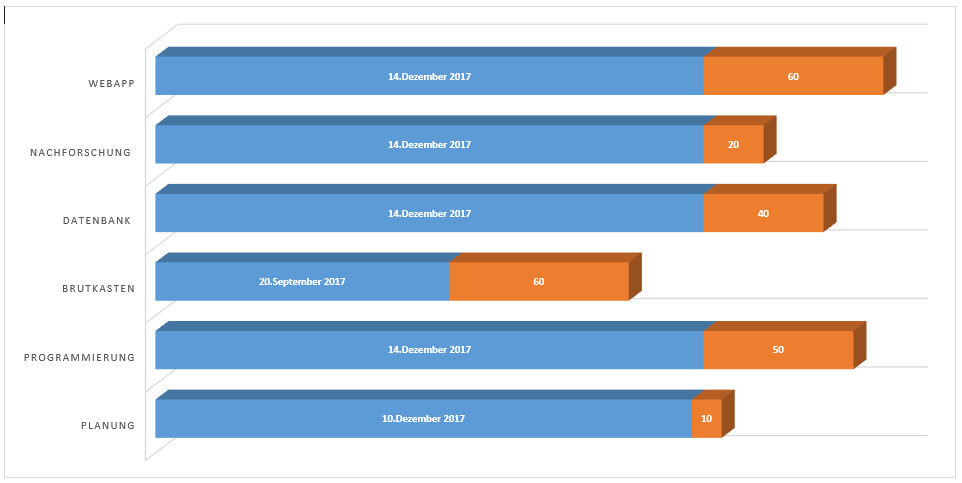
\includegraphics[width=530pt]{figures/Gant}
\caption{Unser Gant Chart für das Projekt} 
\end{figure}
\subsection{Abnahmekriterien}
Die Abnahmekriterien wurden von unserem Auftraggeber so gesetzt das es einen Prototypen geben soll welcher Daten auslesen kann und darauf reagiert.
\subsection{Pläne zur Evaluierung}
Zuerst wollen wird die Daten auf unserem Arduino auslesen und diese dann mithilfe eines Wlan Modul es an unsere Website senden.


\chapter{Vorstellung des Produktes}
Vorstellung des fertigen Produktes anhand von Screenshots, Bildern, Erklärungen.

\chapter{Eingesetzte Technologien} \label{sec:tech}
\begin{itemize}
	\item Kurzbeschreibung aller Technologien, die verwendet wurden.
	\item Technologien die aus dem Unterricht bekannt sind, nur nennen und deren  Einsatzzweck im Projekt beschreiben, nicht die Technologien selbst.
	\item Technologien die aus dem Unterricht nicht bekannt sind, im Detail beschreiben incl. deren Einsatz im Projekt
	\item Fokus aus eingesetzten Frameworks
\end{itemize}

\newpage	
\def \currentAuthor {Florian Tipotsch}
	\section{Technologie für Webapp}
\begin{itemize}
	\item PHP - Für Webapp
	\item Html - Für Webapp 	
	\item MySql - Für Datenbanken
	\item Yii2 - Für Webapp
	\item MVC - Für Webapp
\end{itemize}
	\subsection{MVC - Model, View, Controller}
	\subsection{Was ist MVC?} \label{sec:mvc}
	MVC, auch Model, View, Controller ist ein modernes Entwurfsmuster das meist für Anwendungen die ein User Interface beinhalten. Zum Beispiel für PHP, JAVA, C\# und Ruby Anwendungen. \cite{MVC}
	\subsection{Vor- und Nachteile}
	\begin{tabular}{ l r }
		Vorteile & Nachteile \\
		Gleichzeitiges Programmieren & Schlechte Übersicht \\
		Hohe Kohäsion \cite{kohaesion} & Konsistente Programmierung notwendig\\
		Lose Kopplung \cite{kopplung} & Steile Lernkurve \\	
	\end{tabular}
	\subsection{Yii2}
	\subsubsection{Was ist Yii}
	Yii ist ein high Performance PHP Framework welches vor allem für die Entwicklung im Web2.0 eingesetzt wird. Web 2.0 fördert die User aktiv im Web mitzumachen. Diese können eigenen Beiträge erstellen und diese auf der Website anzeigen lassen.\cite{Web_2}
	
	\subsubsection{Vor- und Nachteile}
	Yii hat sehr viele Vorteile, allerdings auch einig Nachteile:
	Vorteile sind:
	\begin{itemize}
		\item CRUD-Creator (Gii)
		\item Model Generator (Gii)
		\item Einfache Implementierung von HTML Formulare
		\item Einfach Datenbankzugriffe
	\end{itemize}
	\subsubsection{Gii} \label{sec:gii}
	Gii ist der Yii eigene Model, Crud, Controller, Form, Module und Extension Generator. Mit ihm kann man sehr einfach eine Model Klasse mit einer Unterliegenden Datenbanktabelle erstellen. Aus dieser Model klasse kann man dann wiederum CRUD befehle erzeugen. Mit Gii kann man die gesamte Grund MVC Struktur für Yii2 erzeugen und im weiter verlauf dann nach eigenen Wünschen verändern.
	\subsection{Alternative zu Frameworks}
	Yii kann sehr weitreichend eingesetzt werden. Mit dem richtigen Wissen und Fähigkeiten kann man alles was mit einer PHP Seite möglich ist ganz einfach in Yii2 umsetzten.

Allerdings sind Frameworks nicht Administratoren freundlich da sie sehr viel Vorwissen erfordern um diese richtig zu implementieren. Einfacher zu implementieren sind CMS Systeme. Es gibt sehr viele Große CMS Systeme zum Beispiel:
\begin{itemize}
\item Joomla
\item Wordpress
\item Drupal
\item Contao
\end{itemize}
Diese haben wir auch schon im Unterricht besprochen und damit Websites erstellt. Vorteile sind vor allem die einfache Implementierung und rasche Einrichtung einer Website. Auch SEO wird von den CMS Systemen vereinfacht. Nachteile sind allerdings oft eingeschränkte Möglichkeiten und grenzen welches das CMS setzt.

\subsection{Warum haben wir uns für YII2 entschieden}

Der Hauptgrund warum wir uns gegen CMS Systeme entschieden haben sind die eingeschränkten Möglichkeiten die wir damit hätten. Bei YII2 können wir die gesamte Website nach unseren Bedarf zusammenstellen und auch so bearbeiten wie wir es wollen. Es war uns auch wichtig das wir nach modernen Entwurfsmustern arbeiten. Siehe \nameref{sec:mvc}.

Wir hätten uns auch für andere Frameworks entscheiden können allerdings war uns Yii2 schon bekannt und wir haben damit schon einige Websites erstellt.

Alternativen für Yii2 sind:
\begin{itemize}
	\item PureMVC
	\item Laravel
\end{itemize}
\subsection{PureMVC}
PureMVC ist seit dem Release in 2008 unverändert. Das hat den Vorteil das der administrative aufwand sehr gering ist aufgrund nicht vorhandener Updates. Außerdem muss man das Framework nur einmal lernen und kann dieses dann meistern ohne irgendwelche Änderungen zu befürchten.
Es gibt auch Best-Practicse Beispiele in vielen verschiedenen Sprachen. Diese findet man auf der Website \cite{Pure_MVC}
\subsection{Laravel}
Laravel
\newpage
\def \currentAuthor{Kevin Glatz}
\section{Gas-Sensoren}
\subsection{MQ Gas Sensoren}
Es gibt mehrere MQ Gas Sensoren zum Beispiel:
\begin{itemize}
\item {MQ2}
	Methane, Butane, LPG, smoke
\item {MQ3}
	Alcohol, Ethanol, smoke
\item {MQ4}
	Methane, CNG Gas
\item {MQ5}
	Natural gas, LPG
\item {MQ6}
	LPG, butane gas
\item {MQ7}
	Carbon Monoxide
\item {MQ8}
	Hydrogen Gas
\item {MQ9}
	Carbon Monoxide, flammable gasses
\item Mehr gibt es auf der Website: \cite{MQ_Sensoren}
\end{itemize}
In der Schule haben wir den MQ2 zur Verfügung stehend werden wir auch von der Schule den Adafruit CCS811 bereitgestellt bekommen. Wir bedanken uns dafür vielmals.
\newline
{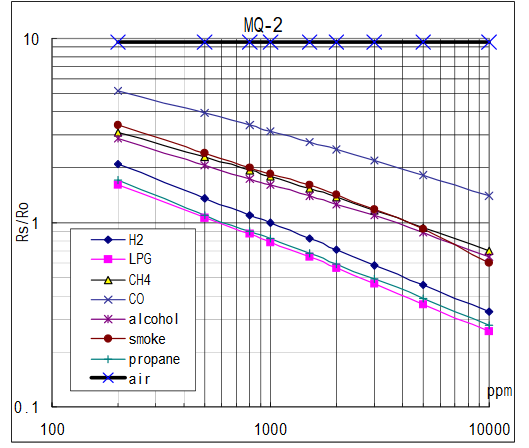
\includegraphics[width=0.8\linewidth]{figures/DatasheetMQ2.png}}{\cite{MQ_Datasheet}}
\cite{MQ_Sensoren}
\newline 
Im Datasheet \cite{MQ_Datasheet} kann man herauslesen das der Sensor MQ2 \cite{MQ_Sensoren} H2, LPG, CH4, CO, Alkohol, Rauch und Propan in einem Bereich von 200 bis 10000 Parts per million (Anteil pro Million) messen kann. Wie empfindlich der Sensor ist, hängt von den RS und RO werten ab.
\begin{itemize}
	\item RS: Sensor Widerstand bei verschiedenen Konzentrationen von Gas
	\item RO: Sensor Widerstand bei 1000ppm von H2 bei sauberer Luft.
\end{itemize}

\subsection{Adafruit CCS811}



\chapter{Problemanalyse}
\section{USE-Case-Analyse}
\begin{itemize}
	\item UseCases auf Basis von Benutzerzielen identifizieren: 
	\begin{itemize}
		\item Benutzer eines Systems identifizieren
		\item Benutzerziele identifizieren (Interviews)
		\item Use-Case-Liste pro Benutzer definieren
	\end{itemize}
	\item UseCases auf Basis von Ereignissen identifizieren: 
	\begin{itemize}
		\item Externes Event triggert einen Prozess
		\item zeitliches Event triggert einen Prozess (Zeitpunkt wird erreicht) 
		\item State-Event (Zustandsänderung im System triggert einen Prozess)
	\end{itemize}
	\item Werkzeuge:
	\begin{itemize}
		\item USE-Case-Beschreibungen (textuell, tabellarisch)
		\item USE-Case-Diagramm
		\item Aktivitätsdiagramm für den Use-Case (Interaktion zwischen Akteur und System abbilden)
		\item System-Sequenzdiagramm (Spezialfall eines Sequenzdiagramms: Nur 1 Akteur und 1 Objekt, das Objekt ist das komplette System, es geht um die Input/Output Requirements, die abzubilden sind)
	\end{itemize}
\end{itemize}

\section{Domain-Class-Modelling}
\begin{itemize}
	\item "Dinge" (Rollen, Einheiten, Geräte, Events etc.) identifizieren, um die es im Projekt geht
	\item ER-Modellierung oder Klassendiagramme
	\item Zustandsdiagramme (zur Darstellung des Lebenszyklus von Domain-Klassen darstellen)
\end{itemize}

\section{User-Interface-Design}
\begin{itemize}
	\item Mockups
	\item Wireframes
\end{itemize}


\chapter{Systementwurf}

\section{Architektur}
\def \currentAuthor{Florian Tipotsch}
\subsection{Design der Komponenten}

Unsere Webapp ist in Yii2 programmiert und ist deshalb nach dem MVC Muster aufgebaut.
\subsection{MVC - Model, View, Controller}\label{sec:MVC}

\subsubsection{Was ist MVC?} 
MVC, auch Model, View, Controller ist ein modernes Entwurfsmuster das meist für Anwendungen die ein User Interface beinhalten, eingesetzt wird. Zum Beispiel für PHP, JAVA, C\# und Ruby Anwendungen. \cite{MVC}

\subsubsection{Vor- und Nachteile}
\begin{tabular}{ l r }
	Vorteile & Nachteile \\
	Gleichzeitiges Programmieren & Schlechte Übersicht \\
	Hohe Kohäsion \cite{kohaesion} & Konsistente Programmierung notwendig\\
	Lose Kopplung \cite{kopplung} & Steile Lernkurve \\	
\end{tabular}

Das MVC Entwurfsmuster ist sehr weit verbreitet und hoch angesehen, es wird deshalb in den meisten Anwendungen mit User Interface angewandt. Der Grund für die Verwendung dieses Musters sind die Vielen Vorteile die es bietet. Außerdem können viel Nachteile über Frameworks behoben werden.

\subsubsection{Aufbau von MVC}
Im Grunde arbeitet MVC mit 3 Klassen:
\begin{itemize}
	\item Modell
	\item View
	\item Controller
\end{itemize}
Die Unterschiedlichen Klassen haben unterschiedliche Aufgaben.

\subsubsection{View}
Die View Klasse ist nur zum Anzeigen der einzelnen Teile des User Interfaces verantwortlich. Bei Webseiten zum Beispiel die Index Seite oder das Login Formular. Außerdem nimmt es alle Benutzer/innen Eingaben entgegen.
\subsubsection{Controller}
Die Controller Klasse Steuert die ganze Anwendung, sie nimmt die User eingaben von der View Klasse entgegen und verarbeitet diese. Außerdem ändert sie auch die View Klasse um andere Seiten anzuzeigen. Sie nimmt auch die Daten von der Modell Klasse entgegen, verarbeitet diese und gibt sie an die View Klasse weiter.
\subsubsection{Modell}
Die Modell Klasse enthält die darzustellenden Daten, sie ist unabhängig von der View und der Controller Klasse

\subsection{CRUD - Create, Read, Update, Delete} \label{sec:CRUD}

\subsubsection{Was ist CRUD?}
CRUD sind die 4 grundlegenden Aufgaben einer Datenbankanbindung:
\begin{itemize}
	\item Create - Erstellen neuer Datensätze
	\item Read - Auslesen der Datensätze
	\item Update - Aktualisieren von vorhandenen Datensätze
	\item Delete - Löschen von Datensätzen
\end{itemize}
\cite{CRUD}
\newline
CRUD ist für alle Datenbankzugriffe verantwortlich die gemacht werden.


\subsection{Yii2} \label{sec:YII2}

\subsubsection{Was ist Yii}
Yii ist ein high Performance PHP Framework welches vor allem für die Entwicklung im Web2.0 eingesetzt wird. Web 2.0 fördert das User aktiv im Web mitmachen. Diese können eigene Beiträge erstellen und diese auf der Website anzeigen lassen.\cite{Web_2}

\subsubsection{Gii} \label{sec:gii}
Gii ist der Yii eigene Model, Crud, Controller, Form, Module und Extension Generator. Mit ihm kann man sehr einfach eine Model Klasse mit einer Unterliegenden Datenbanktabelle erstellen. Aus dieser Model klasse kann man dann wiederum CRUD befehle erzeugen. Mit Gii kann man die gesamte Grund MVC Struktur für Yii2 erzeugen und im weiterm Verlauf dann nach eigenen Wünschen verändern.

\subsubsection{Vor- und Nachteile}
Yii hat sehr viele Vorteile, allerdings auch einig Nachteile:
Vorteile sind:

\begin{itemize}
	\item CRUD-Creator (\nameref{sec:gii})
	\item Model Generator (\nameref{sec:gii})
	\item Einfache Implementierung von HTML Formulare
	\item Einfach Datenbankzugriffe
\end{itemize}

Nachteile ist der Hohe Setup aufwand und die benötigte Kenntnisse in PHP und SQL, welche allerdings bei fast allen Frameworks von Nöten sind.


\subsection{Benutzerschnittstellen} 

Die Benutzerschnittstelle unseres Brutkasten besteht hauptsächlich über die Webapp. Dort kann man sich anmelden und die Daten für den eigenen Brutkasten auslesen. Um sicherzugehen das man nur die eigenen Daten sieht, muss man sich auf der Website mit der Seriennummer die man beim Kauf eines Kasten erhält registrieren. Dadurch kann man dann auf die Daten zugreifen welche für die jeweilige Seriennummer gespeichert sind.
\newline
Wenn man noch nicht registriert wird kann man auf der Website einen Link zu unserem Webshop sehen, den wir allerdings nicht in diesem Projekt erstellen werden da es den Rahmen dieses Projektes Sprengen würde.
\subsection{Datenhaltunskonzept}
Hier ist unser ER-Diagramm
	\begin{figure}
	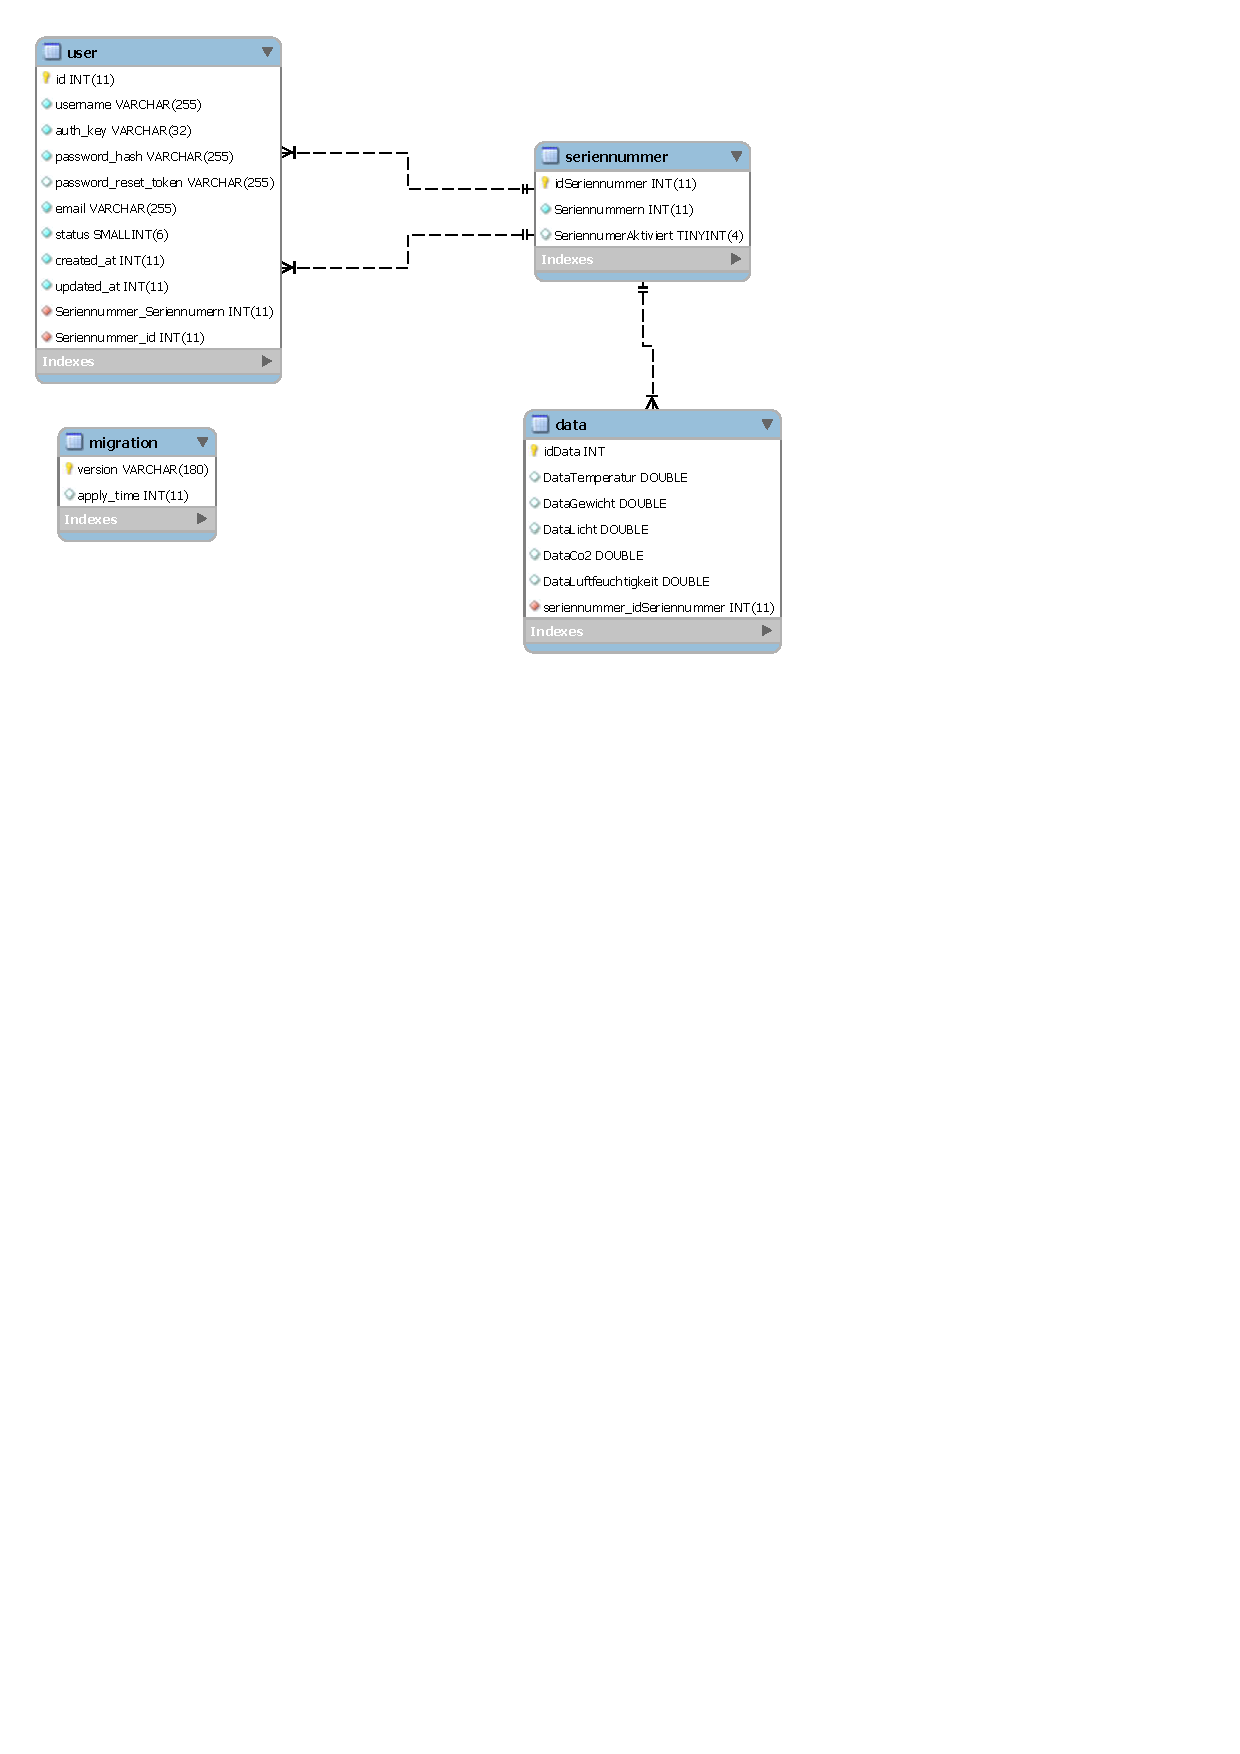
\includegraphics[height=1000pt]{figures/ERDiagramm}
	\caption{ERDiagramm unserer Datenbank}
	\end{figure}
	\newline
	Die Datenbank werden wir bei unserem Web Hoster anlegen und dort alle Daten bis zu 7 Tage Speichern. Daten sollen alle 5-10 Minuten von unserem Brutkasten übermittelt werden. Zur Übermittlung werden wir ein WLAN Modul an unserem Brutkasten anbringen. Mehr dazu im Kapitel \nameref{sec:daten}. Für Prototyp Zwecken werden wir die Daten vorerst lokal über PHPMyAdmin speichern.
	\newpage
	\def \currentAuthor{}
\subsection{Konzept für Ausnahmebehandlung}
\begin{itemize}
	\item Systemweite Festlegung, wie mit Exceptions umgegangen wird
	\item Exceptions sind primär aus den Bereichen UI, Persistenz, Workflow-Management
\end{itemize}
	\newpage
	\def \currentAuthor{Florian Tipotsch}
\subsection{Sicherheitskonzept}

Auf unsere Website kann man sich mithilfe von Username und Password anmelden. Im Weiteren verlauf des Projektes besteht noch die Möglichkeit für unsere Rest Schnittelle eine Authentifizierung einzubauen. Da unser Prototyp allerdings nur lokal vorhanden ist ist dies zum jetzigen Zeitpunk noch nicht notwendig.

\subsection{Design der Testumgebung}
Unseren Protoyp testen wird indem wir ihn einen Tag autonom laufen lassen und am Ende dieser 24h Periode alle Daten kontrollieren ob diese Sinn machen und der Realität entsprechen. Um dies zu gewährleisten bräuchten wir allerdings einen Klima Regulierten Raum der Co2 messen kann.

\subsection{Desing der Ausführungsumgebung}
Das Endprodukt sollte im Freien autonom funktionieren können. Das Setup für den Endbenutzer/in besteht aus dem anstecken an eine Stromversorgung und dem Verbinden mit dem Internet, sowie das einsetzen der Insekten. Im weiteren Verlauf der Brutzeit muss der Benutzer/ die Benutzerin die Insekten füttern. Unser Produkt übernimmt das Regulieren der Temperatur sowie Co2 Werten damit die Insekten Überleben können.

\begin{itemize}
	\item Design-Klassendiagramme vom Domain-Klassendiagramm ableiten (incl. detaillierter Darstellung und Verwendung von Vererbungshierarchichen, abstrakten Klassen, Interfaces)
	\item Sequenzdiagramme vom System-Sequenz-Diagramm ableiten
	\item Aktivitätsdiagramme
	\item Detaillierte Zustandsdiagramme für wichtige Klassen
\end{itemize}

Verwendung von CRC-Cards (Class, Responsibilities, Collaboration) für die Klassen
\begin{itemize}
	\item um Verantwortlichkeiten und Zusammenarbeit zwischen Klassen zu definieren und
	\item um auf den Entwurf der Geschäftslogik zu fokussieren
\end{itemize}

Design-Klassen für jeden einzelnen USE-Case können z.B. sein:

\begin{itemize}
	\item UI-Klassen
	\item Data-Access-Klassen
	\item Entity-Klassen (Domain-Klassen)
	\item Controller-Klassen
	\item Business-Logik-Klassen
	\item View-Klassen
\end{itemize}

Optimierung des Entwurfs (Modularisierung, Erweiterbarkeit, Lesbarkeit):

\begin{itemize}
	\item Kopplung optimieren
	\item Kohäsion optimieren
	\item SOLID
	\item Entwurfsmuster einsetzen
\end{itemize}

\newpage
\def \currentAuthor{Kevin Glatz}

\section{Programmierung}

\subsection{Verkablung}
Die Verkablung der einzelnen Module ist aus verschiedenen Gründen wichtig. Zum einen brauch jedes Modul genügend Strom um seine Aufgabe zu erfüllen, gleichzeitig würde es aber ohne die Erdung zu einem Kurzschluss kommen. Des weiteren ist es wichtig das die Module Daten auslesen und weitersenden können



\subsubsection{Bibliotheken importieren und globale Variablen definieren}

In diesem Schritt importieren wir die nötigen Bibliotheken welche aus GitHub oder direkt von Arduino zur verfügung gestellt bekommen. Auch werden alle Variablen die sowohl in den Methoden Setup und Loop verwendet werden erstellt. 

\subsubsection{Setup}

Die Funktion Setup wird verwendet um einmalige Konfigurationen zu tätigen. Dazu zählen unter anderem Aufbau einer Verbindung, Kalibrierung sensibler Controller oder ähnlichen. Die hier getätigten Aktivitäten werden nur ausgeführt wenn der Arduino startet bzw. zurückgesetzt wird.

\subsubsection{Loop}

Diese Methode verarbeitet und gibt all unsere Werte aus. Besonders an der Klasse Loop ist, dass diese dauerhaft wiederholt wird. Es gibt keine maximale Durchlaufmenge und die Geschwindigkeit eines Durchlaufs wird von der Methode \"delay\" in Millisekunden definiert. Mit Hilfe dieser Eigenschaften, können wir zeitnahe alle Daten auslesen. Falls nun ein Wert eine Mindestgrenze kann sofort darauf reagiert werden. 

Eine genauere Beschreibung der einzelnen Module und deren Programmierung erfolgt in den kommenden Seiten.


\chapter{Implementierung}
Detaillierte Beschreibung der Implementierung aller Teilkomponenten der Software entlang der zentralsten Use-Cases:

\begin{itemize}
	\item GUI-Implementierung
	\item Controllerlogik
	\item Geschäftslogik
	\item Datenbankzugriffe
\end{itemize}

Detaillierte Beschreibung der Teststrategie (Testdriven Development):

\begin{itemize}
	\item UNIT-Tests (Funktional)
	\item Integrationstests
\end{itemize}

Zu Codesequenzen:
\begin{itemize}
	\item kurze Codesequenzen direkt im Text (mit Zeilnnummern auf die man in der Beschreibung verweisen kann)
	\item lange Codesequenzen in den Anhang (mit Zeilennummer) und darauf verweisen (wie z.B. hier)
	
	
\end{itemize}

\def \currentAuthor {Florian Tipotsch}

\section{Webapp}

Für unser Projekt erstellen wir eine Webapp mit der man die Daten seiner eigenen Zuchtkammer anzeigen lassen kann.
Wir haben geplant das man sich mit der Seriennummer der Box Registrieren kann und dann am Handy über eine Webapp alle Daten anzeigen lassen kann. Folgende Daten sollte man auslesen können:

\begin{itemize}
	\item Sauerstoff
	\item Luftfeuchtigkeit
	\item Gewicht
	\item Temperatur
	\item Futtermenge
	\item ungefähre Zeit bis zu Reife
\end{itemize}
Als Grundlage für die Website haben wir das Framework Yii2 verwendet. Mehr dazu im Kapitel \nameref{sec:YII2}.

\subsection{Mockups}
\begin{figure}
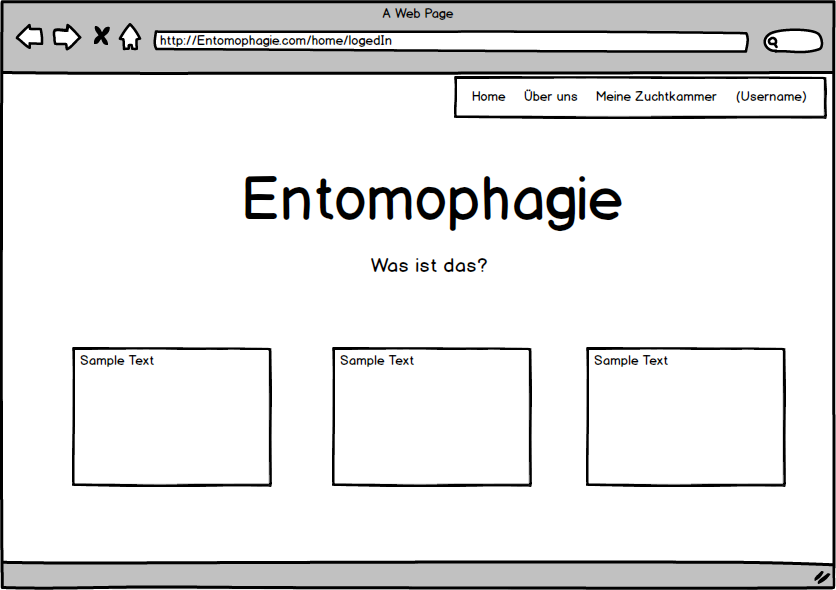
\includegraphics[height=10cm]{figures/Logedin}
\caption{Mockup unserer Seite wenn man eingeloggt ist}
\end{figure}
Hier sieht man die Ansicht wenn man auf unserer Website Angemeldet ist. Man kann auf seine eigene Zuchtkammer zugreifen indem man auf den Button 'Meine Zuchtkammer' klickt und dort die Daten auslesen.
\newpage
\begin{figure}
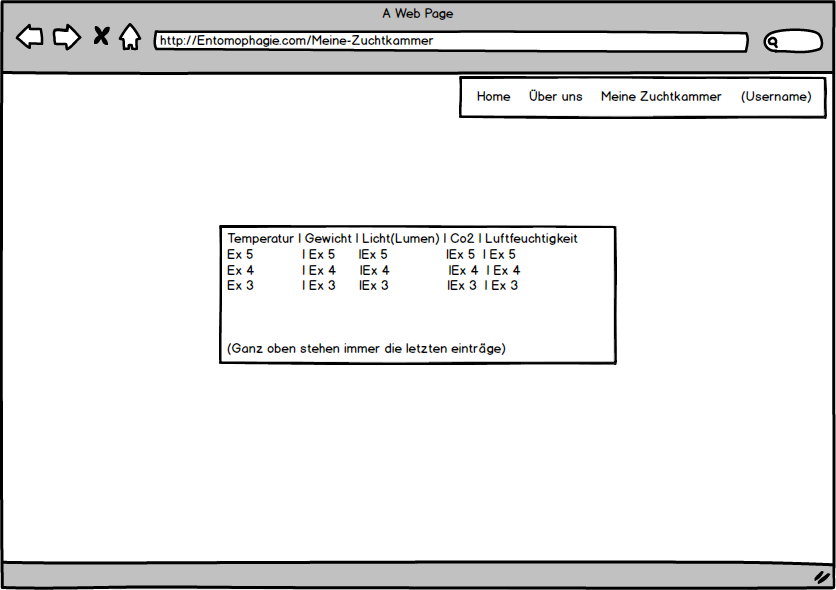
\includegraphics[height=10cm]{figures/Meine-Zuchtkammer}
\caption{Mockup der Seite Meine-Zuchtkammer}
\end{figure}
Auf der Seite 'Meine Zuchtkammer' sieht die letzten Daten die die Zuchtkammer wiedergegeben hat. Diese sind in Absteigender Reihenfolge geordnet,dass heißt, dass der letzte Eintrag ganz oben steht.
\newpage
\begin{figure}
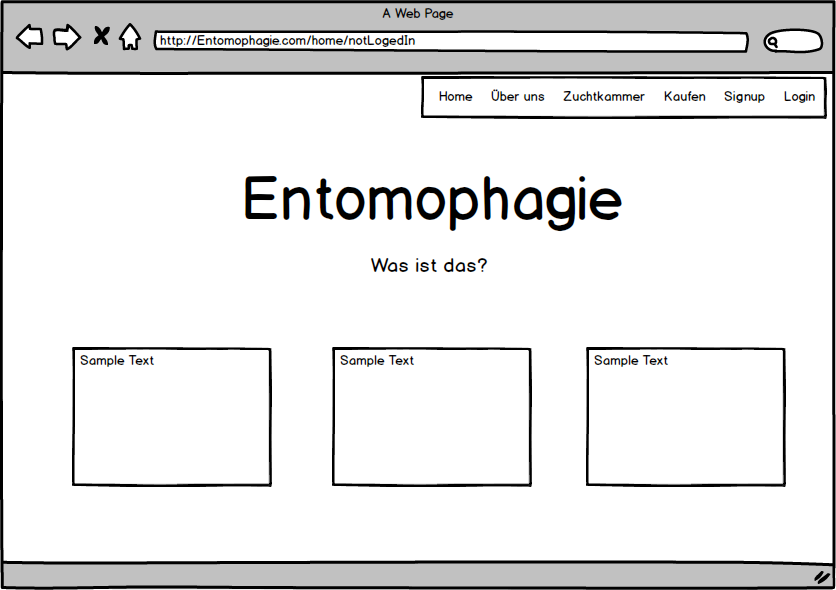
\includegraphics[height=10cm]{figures/NotlogedIN}
\caption{Mockup unserer Seite wenn man nicht eingeloggt ist}
\end{figure}
Hier Sieht man die Ansicht wenn man auf unserer Website nicht Angemeldet ist. Man kann über den Button 'Zuchtkammer' mehr über unsere Zuchtkammern herausfinden, weiter kann man über den Button 'Kaufen' seine eigene Zuchtkammer kaufen. Bei Signup kann man sich als neuer Benutzer registrieren, um sich allerdings zu registrieren brauch man zuerst eine Seriennummer die man beim kauf einer Zuchtkammer erhält.
\newpage

\subsection{Datenbankzugriffe}
Unserer Datenbank zugriffe werden von unserem Framework verarbeite, dabei verwendet das Framework CRUD befehle und arbeitet nach dem MVC Muster. Das heißt es gibt ein unterliegendes Modell welches Daten an unseren Controller mitgibt welche wiederum die View erzeugt.

Der gesamte Datenbankzugriff kann mittels Yii2 sehr einfach erstellt werden. Mehr dazu siehe \nameref{sec:gii}

\subsection{Datenübermittlung} \label{sec:daten}

Um die Daten von unsrem Arduino an unsere Datenbank zu senden werden wir in den Brutkasten ein WLAN Modul einbauen und die Daten alle 5-10 Minuten als JSON-Format an unsere REST-Schnittstelle unserer Webapp senden. Hierfür haben wir das WLAN Modul ESP8266 verwendet. Das hat den Vorteil das unsere Daten direkt von unserem Brutkasten an die Datenbank gegeben werden kann.
\newline
Für diese Lösung brauchen wir eine REST Schnittelle in unserer Webapp. Dies kann über YII2 sehr einfach realisiert werden. Yii2 hat eine vor implementierte REST Schnittelle welche man nur noch aktivieren muss. Die Daten werden aus der Modell Klasse ausgelesen und über den Controller an die REST-View weitergeleitet. Die ganze Implementierung sind 5-10 Zeilen Code. Die Code Sequenz sehen sie im Kapitel \nameref{sec:Rest}.

\subsection{Rest Schnittelle} \label{sec:Rest}
\begin{figure}	
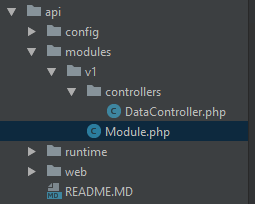
\includegraphics{figures/Ordner}
\caption{Abbildung des API Ordners}
\end{figure}
\newline
Hier sieht man die Ordnerstruktur. Wir erstellen im Obersten Verzeichnis einen neuen Ordner namens 'api' um im Web über folgende \newline URL:'www.entomophagie/api/web/v1/datas' auf unsere Restschnittelle Zugreifen können. Dabei müssen wir darauf achten das wir Groß- und Kleinschreibung beachten. Da es sonst passieren kann das wir keine Anzeige bekommen. Um dieses Problem zu lösen ist es am einfachsten alle Ordner in unserem Verzeichnis immer klein zuschreiben.\newline
Weiters Kopieren wir 'web', 'config' und den 'runtime' Ordner aus unserem Front- bzw. Backend Ordner. 
\begin{lstlisting}[caption=Controller Klasse für REST]
<?php

namespace api\modules\v1\controllers;
use yii\rest\ActiveController;

class DataController extends Active Controller
{
	public $modelClass = 'common\models\Data';
}
\end{lstlisting}

Hier sieht man die Controller Klasse. In der Controller Klasse müssen wir den Yii eigenen ActiveController einbinden und die Modell Klasse festlegen welche die Daten ausliest.
\begin{lstlisting}[caption=Module Klasse für REST]
<?php

namespace api\modules\v1;

class Module extends \yii\base\Module
{
public $controllerNamespace = 'api\modules\v1\controllers';

public FUnction init()
{
	parent::init();
}
}
\end{lstlisting}
Hier sieht man die Module Klasse. In der Module Klasse wird unser neuer Rest Controller initialisiert, damit unsere Anwendung diese Verwenden kann. Dort müssen wir unseren Controller den wir zuvor erstellt haben festlegen.
\newline
Wir haben den Rest Controller mit folgendem Online Tutorial erstellt \cite{Restt}.



\newpage
\section{Arduino}

\def \currentAuthor {Kevin Glatz}
\section{Verkablung}


\subsection{Aufbau}

(bild einfügen)

In Abbildung x können wir nun den Arduino und das Breadboard sehen.  Dort kann man direkt die drei Farben erkennen die jeweils für Stromzufuhr (blau), Datenauslesung (grün) und Erdung (braun) stehen.

(bild mit stromfluss einfügen)

Hier sieht man wie der Strom im Breadboard fließt. Das heißt wenn man in der Untersten Reihe das Board mit 5 Volt versorgt sind alle weiteren Steckplätze verwendbar. Wichtig hierbei ist, dass das Kabel für die Stromzufuhr auch auf der richtigen Reihe platziert wurde. Das erkennt man bei dieser Leiterplatte an dem Plus und Minus Zeichen Plus steht hierbei für Strom und Minus für die Erdung.

Falls man das Falsch verkabelt funktioniert das Modul nicht, es werden allerdings keine Schäden angerichtet


(Bild mit analog und digitalwerten einfügen)

Der Arduino hat zwei Möglichkeiten Daten auszulesen. Einmal spricht man hier von digitaler und analogen Datenauslesung. (internet suche) Digitale Werte bedeutet hier allerdings nur das der ausgelesene Wert als 0 oder 1 abgespeichert werden kann, analoge Daten sind bei diesem Punkt anders, da diese einen Wert zwischen 0 und x haben können (zitat)

\section{Programmierung}

Um die Daten der einzelnen Sensoren verwenden zu können, müssen diese ausgelesen und sinnvoll wiedergegeben werden. Nur sobald die Sensoren richtig Programmiert und verkabelt sind, kriegt man lesbare Information. Diese können anschließend weiter interpretiert und verwendet werden. 
In diesem Projekt kann der Quellcode in drei Bereiche eingeteilt werden. 


\subsection{DHT11 \& CCS811}

Für den DHT 11 sowie dem CCS811 gibt es eine von Adafruit frei verwendbare Bibliothek. Mithilfe von dieser kann man ein Objekt erstellen und es mithilfe diesem Objektes die Momentane Temperatur/Luftfeuchtigkeit auslesen.



Der Parameter \#include fügt externe Klassen in unser Projekt ein und erlaubt es uns in das Objekt dht sowie ccs zu erstellen.
Des weitere können wir mit dem Parameter \#define relevante Daten festlegen. Ein solches Beispiel ist von welchem Pin Daten empfangen werden.


\begin{lstlisting}[language=C, caption=Datenauslesung CCS811, label=code:CCS811read]

delay(2000);
if(ccs.available()){
	if(!ccs.readData()){
		Serial.print("CO2: ");
		Serial.println(ccs.geteCO2());
	}
	else{
		Serial.println("ERROR!");
		//while(1);
	}
}
\end{lstlisting}

\cite{CCS811man}



Die Loop Funktion, wiederholt sich im vorgegebenen Rhythmus immer wieder und gibt keine Variablen zurück. Dort werden alle Daten ausgelesen und an das WLAN Modul weitergeschickt bzw. in diesem Fall wird es auf den Serial Monitor ausgegeben.

Die WENN abfrage prüft als erstes ob der CO2 Sensor kalibriert wurde oder nicht. Falls es gelungen sein sollte gibt es die Werte mit dem Befehl Serial.println(ccs.geteCO2()); im Serial Monitor aus.

\subsection{Hebel}

Das Joystick bzw. der Hebel konnte direkt abgelesen werden. Wichtig hierbei ist es das man nicht nur eine Achse im Setup verwendet sondern beide, ansonsten kommt es bei dem Loop zu einem Fehler und der Wert der benötigten Achse verändert sich nicht.


\subsection{SG90}

Die vom verwendeten Bibliotheken waren bei der Installierung der Arduino eigenen IDE direkt dabei. Die Servo kontrolliert die Luftzufuhr und muss daher Werte vom CCS811 wiederverwenden

\begin{lstlisting}[language=C, caption=Automatisierten Servobewegung bei zu niedrigen CO2 Werten, label=code:SG90]

if(ccs.geteCO2() <= co2Min){
	//move the micro servo from 0 degrees to 180 degrees
	for(;servoAngle < 180; servoAngle++) {       
		servo.write(servoAngle);              
		delay(10);
	} 
} if (ccs.geteCO2() > co2Min && servoAngle != 0){
	servo.write(45); 
	servoAngle = 0;
	Serial.println("RETURN");
}
\end{lstlisting}
\cite{SG90tut}

Die If Abfrage prüft ob CO2 einen Mindestwert (co2Min) unterschreitet. Falls das passiert  wird eine Schleife ausgeführt die den Servo 180° dreht. Diese 180° würde die Lüftungsklappe aufhalten. Falls der CO2 Wert wieder in einem akzeptablen Bereich liegt und die Position des Motors nicht null beträgt, wird die zweite Schleife aktiviert die den Motor zur Position 0 zurückbringt 

\newpage
\def \currentAuthor {Florian Tipotsch}
\newpage
\subsection{Wlan}
Für die Implementierung der Wlan anbiendung haben wir ein ESP8266 verwendet. Das Modul ist sehr einfach einzurichten das ganze haben wir mit den Beispielen von den ESP8266 in der Arduino IDE gemacht.

\subsection{ESP8266}
Das Wlan Modul ESP866 wird verwendet um die Verbindung mit dem Internet aufzubauen und die Daten mithilfe der Rest Schnittelle an unsere Website senden. Dafür haben wir die ESP8266 Library von Arduino verwendet.\cite{esp8266}
\begin{lstlisting}[caption=Verbindungsaufbau des ESP8266]
	#include <ESP8266.h>
	
	const char* ssid = "SSID des Benutzers";
	const char* password = "password des Benutzers";
	
	const char* host = "Unsere Website";
	
	void setup(){
	Serial.begin(115200);
	dela(10);
	
	Serial.println();
	Serial.println();
	Serial.println("Connecting to ");
	Serial.println(ssid);
	
	
	WiFi.mode(WIFI_STA);
	WiFi.begin(ssid,password);
	}
\end{lstlisting}

Hier sieht man den Verbindungsaufbau des ESP8266. In der Zeile WIFI.begin wird dann die Verbindung gestarted vorher übergeben wir die SSID und das Password des WLAN womit das Modul sich verbinden soll.
\newpage
\begin{lstlisting}[caption=Verbindungsaufbau Response]
	while(WiFi.status() != WL_CONNECTED) {
	delay(500);
	Serial.print(".");
	}
	
	Serial.println("");
	Serial.println("WiFi connected");
	Serial.println("IP adress: ");
	Serial.println(WiFi.localIP());
	
	


\end{lstlisting}

Bei erfolgreicher Verbindung wird die IP Adresse unseres Moduls ausgegeben.

\begin{lstlisting}[caption=Ausführung der REST Befehle]
client.print(String("GET ) + url + " HTTP/1.1\r\n)" +
	"Host: " + host + "\r\n" + 
	"Connection: close\r\n\r\n");
unsigned long timeout = millis();
while(millis() - timeout > 5000) {
	Serial.println(">>> Client Timeout !");
	client.stop();
	return;
}
\end{lstlisting}
Anschließend können wir in unserer Loop REST Befehle wie Get, Post, Put, etc ausführen.




\chapter{Deployment}
\begin{itemize}
	\item Umsetzung der Ausführungsumgebung
	\item Deployment
	\item DevOps-Thema
\end{itemize}

\chapter{Tests}

\section{Systemtests} 
Systemtests aller implementierten Funktionalitäten lt. Pflichtenheft
\begin{itemize}
	\item Beschreibung der Teststrategie
	\item Testfall 1
	\item Testfall 2
	\item Tesfall 3
	\item …
\end{itemize}

\section{Akzeptanztests}

\chapter{Projektevaluation}
siehe Projektmanagement-Unterricht

\chapter{Benutzerhandbuch} 
falls im Projekt gefordert

\newpage
\chapter{Betriebswirtschaftlicher Kontext}


\def \currentAuthor {Kevin Glatz}
\subsection{Arduino in der Wirtschaft}
Mikrocontroller gewinnen vor allem beim Endverbraucher immer mehr an Qualität, allerdings wird auch im Landwirtschaftlichen Bereich von diesen Technologien Gebrauch gemacht. In dem Artikel \"Arduino Projekte in der Landwirtschaft und Fischzucht\" wird beschrieben wie Privatpersonen ihre eigene Lösung zu Problemen wie Fischzucht, Lenksysteme für Erntemaschinen und weitere Fälle gestalten. 
\cite{ArdAgra}

Für einen Insekten Zuchtkasten existiert in der westlichen Welt keine große Nachfrage, im Asiatischen Raum könnte ein solches Produkt hingegen große Popularität gewinnen. In der Kostenrechnung werden die einzelnen Teile nochmals genauer besprochen, allerdings ist der Anschaffungswert alle benötigten Teile unter € 100. 

\subsection{Kostenrechnung}

\Section{Nutzen einer Website}
Es ist immer wichtiger für Unternehmen eine Website zu besitzen den für viele Personen ist das Internet der erste Ansprechpartner um Informationen zu erhalten. Dabei ist es wichtig das man die gewünschte Website schnell und einfach findet. Dafür ist eine gute Search engine optimation(SEO) wichtig, damit die Website in Google auf der Ersten Seite angezeigt wird. Das ist deshalb wichtig da die zweite Ergebnis Seite von Google oft ignoriert wird.

Auch in unserem Projekt haben wir eine Website erstellt, diese ist allerdings eine Reine Funktionswebsite. Deshalb kann man auf unserer Website erst nur Daten seines Brutkasten auslesen. Man könnte die Website noch mit einem Webshop erweitern, da dies allerdings den Rahmen des Projektes sprengen würde haben wir dies nicht gemacht.

Auf Websiten ist es auch wichtig dass das Unternehmen widergespiegelt wird, deshalb sollte man dort möglichst ein Corporate Design anwenden falls eines vorhanden ist. Den in der heutigen Modernen Zeit ist es für viele der Erste Eindruck über ein Unternehmen.

<<<<<<< HEAD

=======
>>>>>>> 54e20bb2c86065d713b6bc9c404b8e7788b12287


\chapter{Zusammenfassung}
\begin{itemize}
	\item Etwas längere Form des Abstracts
	\item Detaillierte Beschreibung des Outputs der Arbeit
\end{itemize}